\clearpage
\section{\sys{} Suite}
\label{app:suite}

\sys{} suite is the benchmark dataset of six distributed key-value-store specifications we release alongside the system; together with Chapar's published causal-consistency spec~\cite{chapar}, they form the seven specifications evaluated in \cref{sec:eval}. Each specification fixes (i) the abstract spec state and operations the application sees, (ii) the concrete replica state and operations the implementation runs, and (iii) the consistency property the implementation must satisfy. This appendix gives the formal definition of every spec, plus the reference implementations we benchmark in \cref{sec:eval}. The framework setup below introduces the notation: client programs (\cref{fig:prog-def}), the seven-method \texttt{AlgDef} interface (\cref{fig:alg-def}), the configuration syntax (\cref{fig:configuration-syntax}), the concurrent operational semantics (\cref{fig:updated-conc-op-sem}), the refinement hierarchy (\cref{fig:refinement-hierarchy}), and a relaxed baseline spec (\cref{fig:relaxed-specification}).

\paragraph{Summary.}
\Cref{tab:suite-summary} lists the six \sys{} suite specifications plus Chapar's published CC. Each is then introduced in plain English and immediately followed by its formal definition and reference implementation.

\begin{table}[h]
\centering
\small
\setlength{\tabcolsep}{6pt}
\renewcommand{\arraystretch}{1.15}
\begin{tabular}{@{}llp{0.45\linewidth}@{}}
\toprule
spec & abbreviation & informal guarantee \\
\midrule
Read-Your-Writes                          & RYW    & A client's read sees that client's own most recent write. \\
Monotonic Reads                           & MR     & A client's reads never go back in time relative to writes the client has already seen. \\
Monotonic Writes                          & MW     & Writes from one client are applied in order at every replica. \\
Read-Your-Writes $+$ Monotonic Writes     & RYW+MW & Composition of RYW and MW; an implementation must refine both. \\
Causal Consistency                        & CC     & A read returns a value whose causal predecessors have all been observed at the responding replica. \\
Labeled Causal Consistency                & LCC    & CC parameterised by per-message topic labels: each client subscribes to a subset of labels and only sees causality enforced on those. \\
Chapar Causal Consistency                 & Chapar CC & Chapar's published CC specification~\cite{chapar}; see the original paper for its formal definition. \\
\bottomrule
\end{tabular}
\caption{The six \sys{} suite specifications, plus Chapar's published CC for reference.}
\label{tab:suite-summary}
\end{table}
\newpage
% --- Framework setup figures (programs, AlgDef interface, op-sem, refinement, relaxed spec) ---
% 
\usepackage{mathpartir}

\usepackage{graphicx}

% \usepackage[firstpage]{draftwatermark}
% % \SetWatermarkText{\hspace*{8in}\raisebox{3.5in}{\includegraphics[scale=0.1]{aec-badge-popl.pdf}}}
% \SetWatermarkText{\hspace*{13.3in}\raisebox{-6.5in}{\includegraphics[scale=0.1]{aec-badge-popl.pdf}}}
% \SetWatermarkAngle{0}

%--------------------------------------
% To use \mathbb
\usepackage{amsfonts}
%--------------------------------------
% To defined theorems and Lemmas
 \usepackage{amsthm} 
\theoremstyle{definition}  % non-italic
% Definition, Lemma and Theorem
\newtheorem{definition}{Definition}
\newtheorem{theorem}{Theorem}
% \newtheorem{definition}{Lemma}
\newtheorem{lemma}{Lemma}
\newtheorem{corollary}{Corollary}
%--------------------------------------
% To have colored annotations
\usepackage{xcolor}
%--------------------------------------
% To strike out text
\usepackage[normalem]{ulem}
\usepackage{cancel}
%--------------------------------------
%\usepackage{hyperref}
\usepackage{url}
%--------------------------------------
% Programming language rules
\usepackage{mmm}
\usepackage{pl}
%--------------------------------------
% Arrow symbols 
\let\Bbbk\relax
\usepackage{amssymb}
%--------------------------------------
% \xrightarrow
\usepackage{amsmath}
%--------------------------------------
% % To write algorithms
% \usepackage{algorithm}
% %\usepackage{algpseudocode}
% \usepackage[noend]{algpseudocode}
% \let\algState\State
% \usepackage{varwidth}% http://ctan.org/pkg/varwidth
% % To have Algorithm float
% % \usepackage{algorithm}
% % To make the algorithms float to the top
% \usepackage{float}
% \newfloat{algorithm}{t}{lop}
% %\renewcommand{\algorithmicforall}{\textbf{foreach}}
%--------------------------------------

% this employs smarter hyphenations, par, and other rules
% ... and helps condense the paper
\usepackage{microtype}

% To remove a warning for fonts
% \usepackage{lmodern}% http://ctan.org/pkg/lm

%--------------------------------------
% Symbol definitions and comments
% Standard
\def\t{\phantom{X}}

\def\<{\langle}
\def\>{\rangle}

%--------------------------------------

\usepackage{listings}
\lstset{
   language=C,
   captionpos=b,
   tabsize=3,
%   frame=lines,
%   keywordstyle=\color{blue},
%   commentstyle=\color{darkgreen},
%   stringstyle=\color{red},
   numbers=left,
   numberstyle=\tiny,
   numbersep=5pt,
   breaklines=true,
   showstringspaces=false,
%   basicstyle=\small\bfseries,
   basicstyle=\small\ttfamily,
   emph={label}
}

\usepackage{array}

\usepackage{tikz}
\usetikzlibrary{positioning} 
\usetikzlibrary{arrows} 
%\usetikzlibrary{graphs} % Not supported by tikz 2.10
\usetikzlibrary{calc}
\usetikzlibrary{backgrounds}
\usetikzlibrary{shapes}

%\usepackage{caption}
%\usepackage{subcaption}

\usepackage{stmaryrd}

\def\defeq{\triangleq}

\def\self{\mathit{self}}

\def\switch{\mathsf{switch} \ }
\def\case{\mathsf{case} \ }
\def\ret{\mathsf{ret} \ }
\def\lforall{\mathsf{forall} \ }
\def\lif{\mathsf{if} \ }
\def\lelse{\mathsf{else} \ }
\def\lmap{\mathsf{map} \ }
\def\llet{\mathsf{let} \ }
\def\max{\mathsf{max}}

\def\vc{\mathit{vc}}
\def\List{\mathsf{List}}
\def\llookup{\mathsf{lookup} \ }

\def\RYW{\mathit{RYW}}
\def\MR{\mathit{MR}}
\def\WFR{\mathit{WFR}}
\def\MW{\mathit{MW}}
\def\CC{\mathit{CC}}
\def\LCC{\mathit{LCC}}
\def\Rel{\mathit{Rel}}

\def\ext{\mathsf{ext}}

\def\CState{\mathsf{CState}}
\def\RState{\mathsf{RState}}

\def\true{\mathsf{true}}
\def\Set{\mathsf{Set}}
\def\Nat{\mathsf{Nat}}
% \def\L{\mathsf{L}}
\def\L{L}
\def\lab{\mathit{label}}
\def\clientLabs{\mathit{client\text{-}labels}}

\def\cInit{\mathsf{c\text{-}init}}
\def\rInit{\mathsf{r\text{-}init}}

\def\get{\mathsf{get}}
\def\getGuard{\mathsf{get\text{-}guard}}
\def\getReq{\mathsf{get\text{-}req}}
\def\getRes{\mathsf{get\text{-}res}}

\def\lput{\mathsf{put}}
\def\putGuard{\mathsf{put\text{-}guard}}
\def\putReq{\mathsf{put\text{-}req}}
\def\putRes{\mathsf{put\text{-}res}}

\def\Type{\mathsf{Type}}
\def\Option{\mathsf{Option}}
\def\Bool{\mathsf{Bool}}

\def\Event{\mathit{Event}}
\def\Req{\mathit{Req}}
\def\req{\mathit{req}}

\def\Res{\mathit{Res}}
\def\res{\mathit{res}}

\def\PutReq{\mathit{Put\text{-}req}}
\def\PutReqPayload{\mathsf{Put\text{-}req\text{-}payload}}
\def\PutRes{\mathit{Put\text{-}res}}
\def\PutResPayload{\mathsf{Put\text{-}res\text{-}payload}}

\def\GetReq{\mathit{Get\text{-}req}}
\def\GetReqPayload{\mathsf{Get\text{-}req\text{-}payload}}
\def\GetRes{\mathit{Get\text{-}res}}
\def\GetResPayload{\mathsf{Get\text{-}res\text{-}payload}}

\def\Unit{\mathsf{Unit}}

% Program Syntax

% Uses:
% $
% \sPut{}{},
% \sPut{k}{v},
% \sPut[i]{k}{v},
% % 
% \sGet{}{},
% \sGet{x}{k},
% \sGet[i]{x}{k},
% $

\newcommand\sPut[3][]{%
  \mathit{put}%
  \ifthenelse{\equal{#1}{}}{%
    \ifthenelse{\equal{#2}{}}{}{
    ({#2},{#3})}%
  }{%
    ^{#1}({#2},{#3})%
  }%
}  
  
\newcommand\sGet[3][]{%
   \ifthenelse{\equal{#2}{}}{}{#2\leftarrow}%
   \mathit{get}
   \ifthenelse{\equal{#1}{}}{}{^{#1}}%
   \ifthenelse{\equal{#3}{}}{}{({#3})}}

% \newcommand\sGet[2][]{%
%     \ifthenelse{\equal{#1}{}}{}{#1\leftarrow }%
%     \mathit{get}%
%     \ifthenelse{\equal{#2}{}}{}{({#2})}}
    
  \newcommand\sSkip{\mathit{skip}}

\newcommand{\name}[1]{\textsc{#1}}

\newcommand\indrule[3][]{%
%  \inferrule*[Right=#1]{#2}{#3}%
  \inferrule[#1]{#2}{#3}%
  }

\newcommand\figurealgtextsize{%
%   \small%
  \setlength{\abovedisplayskip}{0pt}%
  \setlength{\abovedisplayshortskip}{0pt}%
  \setlength{\belowdisplayskip}{0pt}%
  \setlength{\belowdisplayshortskip}{0pt}}
\newcommand\figureruletextsize{%
%   \small
  \setlength{\abovedisplayskip}{0pt}%
  \setlength{\abovedisplayshortskip}{0pt}%
  \setlength{\belowdisplayskip}{0pt}%
  \setlength{\belowdisplayshortskip}{0pt}
}
\newcommand\figuredefstextsize{%
%   \small
%  \large  
  \setlength{\abovedisplayskip}{0pt}%
  \setlength{\abovedisplayshortskip}{0pt}%
  \setlength{\belowdisplayskip}{0pt}%
  \setlength{\belowdisplayshortskip}{0pt}
}

\usepackage{siunitx}  % To format numbers

\setlength{\textfloatsep}{20pt}

\usepackage{balance}

% \newfont{\mycrnotice}{ptmr8t at 7pt}
% \newfont{\myconfname}{ptmri8t at 7pt}
% \let\crnotice\mycrnotice%
% \let\confname\myconfname%

\newcommand\world[3]{%
   {\begin{array}{l} ( %\left(
      #1, \\ \phantom{(}
      #2, \\ \phantom{(}
      #3          
   ) \end{array}}
}  

\newcommand\note[1]{\text{\small#1}}
\newcommand\bnote[1]{\textbf{\small#1}}

% \newcommand\note[1]{\footnotesize\text{#1}}
% \newcommand\bnote[1]{\footnotesize\textbf{#1}}

\usepackage{tikz}
\usetikzlibrary{positioning, arrows.meta}

%
%
% \begin{document}
%
% \title{Distributed Key-Value Store Specifications and Implementations}
%
% \author{Draft. M. Lesani}
% % \affiliation{%
% %   \institution{University of Example}
% %   \city{Springfield}
% %   \country{USA}
% % }
% % \email{jane.doe@example.edu}
%
% \begin{abstract}
% ...
% \end{abstract}
% \maketitle
% \pagestyle{plain}

% Visual styling for spec figures: subtle pale-gray background and a thin
% light-gray border, matching counter-listing.tex (Fig 1).  The \specfig
% wrapper takes the math content and frames it without altering any of the
% notation inside.
\providecolor{specbg}{HTML}{F7F8FA}
\providecolor{specrule}{HTML}{C8CDD3}
\newcommand{\specfig}[1]{%
  {\setlength{\fboxsep}{4pt}\setlength{\fboxrule}{0.3pt}%
   \fcolorbox{specrule}{specbg}{#1}}%
}



\begin{figure}[h]
\centering
\specfig{%
\begin{minipage}{0.90\linewidth}
  \figuredefstextsize
  \setlength{\abovedisplayskip}{0pt}%
  \setlength{\abovedisplayshortskip}{0pt}%
  \setlength{\belowdisplayskip}{0pt}%
  \setlength{\belowdisplayshortskip}{0pt}%
   \begin{mathpar}
      \begin{array}{rcl@{\qquad}l}
      k
         & : &
            K  % = \Nat
         & 
         \mbox{Key}
      \\
      v
         & : &
            V ⊇ K
         & 
         \mbox{Value}
      \\
      x
         & : &
            V
%             K \ | \ V
         & 
         \mbox{Variable}
      \\
      i
         & &
            
%             K \ | \ V
         & 
         \mbox{Unique Identifiers}
      \\
      s : S
%          & : &
%             S
%          & 
%          \mbox{Statement}
%       \\
         & ::= &
%             \sPut{k}{v} ; \ s
            \sPut[i]{k}{v} ; \ s
         &
         \mbox{Statement}
      \\ & | &
         \sGet[i]{x}{k}; \ s
         &
      \\ & | &
         \sSkip
         &
      \\ & | &
         &
         \mbox{Extended Syntax for Internal Statements}
      \\ & | &
         ⊘ \, \sGet[i]{x}{k}; \ s
         &
         \mbox{Blocked Get}
   \\
   c
      & : &
         C
      & 
      \mbox{Clients}
   \\
      a 
         & : &
            A = C ↦ S
      &
      \mbox{Application}            
      \end{array}
   \end{mathpar}
\end{minipage}%
}
   \caption{\label{fig:prog-def}Client Programs}
\end{figure}

\ \\
\ \\

\begin{figure}[h]
\centering
\specfig{%
\resizebox{0.92\linewidth}{!}{%
\begin{minipage}{1.05\linewidth}
  \figuredefstextsize
  \setlength{\abovedisplayskip}{0pt}%
  \setlength{\abovedisplayshortskip}{0pt}%
  \setlength{\belowdisplayskip}{0pt}%
  \setlength{\belowdisplayshortskip}{0pt}%
   \begin{mathpar}
      \begin{array}{lr}
         𝐈 = (\CState, \cInit, \RState, \rInit,
         & \note{Implementation}
      \\ \phantom{𝐈 = (}
         \getReq, \getGuard, \get, \getRes, 
      \\ \phantom{𝐈 = (}         
         \putReq, \putGuard, \lput)
%          \putRes
   
      \\
         C
         & 
         \note{Clients}
      \\
         \CState : \Type
         & \note{Client State}
      \\
         \cInit : C → \CState
         & \note{Client Initial State}
      \\
         R
         &
         \note{Replicas}         
      \\
         \RState : \Type
         & \note{Replica State}
      \\
         \rInit : R → V → \RState
         & \note{Replica Initial State}
      \\
         \GetReqPayload, \GetResPayload: \Type
         & \note{Get Payload Types}
      \\
% Get
         \getReq : (K) (C, \CState) → 
         (\GetReqPayload, \CState)
         & \note{Get Request (at client)}
      \\
         \getGuard : (K) (\GetReqPayload) (C, R, \RState) → \Bool
         & \note{Get Guard (at replica)}
      \\
         \get : (K) (\GetReqPayload) (C, R, \RState) → 
         (V × \GetResPayload, \RState)
         & \note{Get (at replica)}
      \\
         \getRes : (K, V) (\GetResPayload) (C, \CState) → \CState
         & \note{Get Response (at client)}
      \\
% Put
         \PutReqPayload: \Type
         & \note{Put Payload Type}
      \\
         \putReq : (K, V) (C, \CState) → 
         (\PutReqPayload × \CState)
         & \note{Put Request (at client)}
      \\
         \putGuard : (K, V) (\PutReqPayload) (C, R, \RState) → \Bool
         & \note{Put Guard (at replica)}
      \\
         \lput : (K, V) (\PutReqPayload) (C, R, \RState) → \RState
%          (\RState × \PutResPayload)
         & \note{Put (at replica)}
%       \\
%          \putRes : (C, \CState)(K, V, \PutResPayload) → \Unit
%          & \note{Put Response}
      \end{array}
   \end{mathpar}
\end{minipage}%
}}
   \caption{\label{fig:alg-def}
      Key-Value Store Implementation Interface}
\end{figure}

\clearpage
\begin{figure}[t]
\centering
\specfig{%
\begin{minipage}{0.90\linewidth}
  \figureruletextsize
  \setlength{\abovedisplayskip}{0pt}%
  \setlength{\abovedisplayshortskip}{0pt}%
  \setlength{\belowdisplayskip}{0pt}%
  \setlength{\belowdisplayshortskip}{0pt}%
\figuredefstextsize
\centering
$
\begin{array}{rcl@{\qquad}l}
   𝐈 & = &
      (\CState, \cInit, \RState, \rInit, 
      & \note{Implementation}
   \\ 
      & & \phantom{(}
      \getReq, \getGuard, \get, \getRes, 
   \\   
      & & \phantom{(}
      \putReq, \putGuard, \lput)
   \\
   W  : 𝓦 
      & ≔ &
         〈𝓒, 𝓡, 𝓝 〉
   %             𝓦  = 𝓒 × 𝓡  × 𝓝 
      &
      \mbox{World}
   \\
   c
      & : &
         C
      & 
      \mbox{Clients}
   \\
   σ
      & : &
         \CState
      & 
      \mbox{Client State}
   \\
   𝓒
      & : &
         C ↦ 〈\CState, S〉
      &
      \mbox{Client Programs}
   \\
   r
      & : &
         R
      &
      \mbox{Replicas}
   \\
   ς
      & : &
         \RState
      & 
      \mbox{Replica State}         
   \\
   𝓡 
      & : &
         R ↦ \RState
      & 
      \mbox{Replica States}
   \\
   𝓝
      & : &
         \mathbb{PM}(M)
      &
      \mbox{Network}
   \\
   M
      & : &
      C × R × \GetReq(I, K, \GetReqPayload)
      & 
      \mbox{Message}
   \\
      & | &
      R × C × \GetRes(I, K, V, \GetResPayload)
   \\
      & | &
      C × R × \PutReq(K, V, \PutReqPayload)      
%    \\
%    e
%       & : &            
%          \Event = \Req \ | \ \Res
%       & 
%       \mbox{Event}
%    \\
%    \req : \Req
%       & ≔ &
%          \PutReq( k, v, p )
%          \ | \
%          \GetReq( i, k, p )
%       & 
%       \mbox{Request}
%    \\
%    \res : \Res
%       & ≔ &
%       \PutRes( )
%       \ | \
%       \GetRes( i, k, v, p )
%       & 
%       \mbox{Response}
   \\
   l
      & ::= &
      c ▹ \sGet[i]{}{k}
      & 
      \mbox{Label}
   \\ & | &
      r ▹ \sGet[i]{}{k}: v
   \\ & | &
      c ▹ \sGet[i]{}{k}: v
   \\ & | &
      c ▹ \sPut{k}{v}
   \\ & | &
      r ▹ \sPut{k}{v}
      &
   %       \\ & | &
   %          \mathit{assertfail}  % n ▹ 
   %          &
   \\
   h
      & ::= &
         l ⃰
      & 
      \mbox{History}
   \\
   \ext(h)
      & ::= &
         h \ | \ \{ c ▹ \sGet[i]{}{k}: v, \ c ▹ \sPut{k}{v} \}
      & 
      \mbox{External History}               
   \end{array}
$

\ \\
\ \\

$
%    \vspace{-0.5em} \\
   \begin{array}{rcl}
   ○ & : & \Unit
   \\
   \mathbb{PM}(S)
      & \defeq &
      \mbox{The multiset powerset of the set $S$}
   \\
      W₀(a)_{𝐈}
      & \defeq &
      〈[\overline{c ↦ 〈\cInit(c), a(c)〉}_{c ∈ C}],
         [\overline{r ↦ \rInit(r, v₀)}_{r ∈ R}],
         ∅〉
   %          \mbox{Initial Conf}
   \\
      v_0
      & \defeq &
      \mbox{The initial value}
%       
%    \\[0.5em]
%    \mathbb{P}(S)
%       & \defeq & 
%    \mbox{The powerset of the set $S$}
   \end{array}
$
\end{minipage}%
}

\caption{The State of the Key-value Store Operational Semantics}
\label{fig:configuration-syntax}

\end{figure}

\clearpage
\begin{figure}
% \begin{figure}[t]
\centering
\specfig{%
\begin{minipage}{0.90\linewidth}
  \figureruletextsize
  \setlength{\abovedisplayskip}{0pt}%
  \setlength{\abovedisplayshortskip}{0pt}%
  \setlength{\belowdisplayskip}{0pt}%
  \setlength{\belowdisplayshortskip}{0pt}%
  \begin{mathpar}
      \indrule[Get-Req] {
         c ≠ c₀
         \\\\ 
         \getReq (k) (c, σ) ⇝ ⃰  〈p, σ'〉
      } {
         \world{
            𝓒 [c ↦ 〈σ, \sGet[i]{x}{k}; s〉]
         }{
            𝓡 
         }{
            𝓝
         }
         \xrightarrow{c \ ▹ \ \sGet[i]{}{k}}_{𝐈}
         \world{
            𝓒 [c ↦ 〈σ', ⊘ \, \sGet[i]{x}{k}; s〉]
         }{
            𝓡 
         }{
            𝓝  ∪ \{ \overline{〈c, r, \GetReq(i, k, p)〉 }_{r ∈ R}  \}
         }
      }
      
      \indrule[Get] {
         \getGuard (k) (p) (c, r, ς) ⇝ ⃰  \true
         \\\\
         \get (k) (p) (c, r, ς) ⇝ ⃰  〈v, p', ς'〉
      } {
         \world{
            𝓒 
         }{
            𝓡 [r ↦ ς]
         }{
            𝓝 ∪ \{〈 c, r, \GetReq(i, k, p) 〉 \}
         }
         \xrightarrow{r \ ▹ \ \sGet[i]{}{k} : v}_{𝐈}
         \world{
            𝓒
         }{
            𝓡 [r ↦ ς']
         }{
            𝓝  ∪ \{ 〈 r, c, \GetRes( i, k, v, p' ) 〉\}
         }
      }
   
      \indrule[Get-Res] {
         \getRes (k, v) (p) (c, σ) ⇝ ⃰  σ'
      } {
         \world{
            𝓒 [c ↦ 〈σ, ⊘ \, \sGet[i]{x}{k}; s〉]
         }{
            𝓡 
         }{
            𝓝 ∪ \{〈r, c, \GetRes(i, k, v, p)〉 \}
         }
         \xrightarrow{c \ ▹ \ \sGet[i]{}{k} : v}_{𝐈}
         \world{
            𝓒 [c ↦ 〈σ', s[v / x]〉]
         }{
            𝓡 
         }{
            𝓝  
         }
      }

      \indrule[Put-Req] {
         c ≠ c₀
         \\\\      
         \putReq (k, v) (c, σ) ⇝ ⃰ 〈p, σ'〉
      } {
         \world{
            𝓒 [c ↦ (σ, \sPut{k}{v}; s)]
         }{
            𝓡 
         }{
            𝓝 
         }
         \xrightarrow{c \ ▹ \ \sPut{k}{v}}_{𝐈}
         \world{
            𝓒 [c ↦ (σ', s)]
         }{
            𝓡 
         }{
            𝓝 ∪ \{ \overline{〈c, r, \PutReq( k, v, p )〉 }_{r ∈ R}  \}
         }
      }
   
      \indrule[Put] {
         \putGuard (k, v) (p) (c, r, ς) ⇝ ⃰  \true
         \\\\
         \lput (k, v) (p) (c, r, ς) ⇝ ⃰  ς'
      } {
         \world{
            𝓒 
         }{
            𝓡 [r ↦ ς]
         }{
            𝓝  ∪ \{ 〈c, r, \PutReq( k, v, p ) 〉\}
         }
         \xrightarrow{r \ ▹ \ \sPut{k}{v}}_{𝐈}
         \world{
            𝓒 
         }{
            𝓡 [r ↦ ς']
         }{
            𝓝 
         }
      }
   \end{mathpar}
\end{minipage}%
}
   \caption{\label{fig:updated-conc-op-sem}
      Key-value Store Operational Semantics $→_{𝐈}$
      for the implementation      
      $𝐈 =$ $(\CState,$ $\cInit,$ $\RState,$ $\rInit,$
         $\getReq,$ $\getGuard,$ $\get,$ $\getRes,$
         $\putReq,$ $\putGuard,$ $\lput)$.         
   }
\end{figure}

The $\sGet{}{}$ operations are synchronous. 
Therefore, the semantics implicitly preserves the order of $\sGet{}{}$s and succeeding $\sGet{}{}$s and $\sPut{}{}$s.
% (\textit{i.e.}, total-load order).

\clearpage

\begin{definition}[Trace Inclusion]
An implementation $𝐈₂$ trace-includes another $𝐈₁$, written $𝐈₂ ⊑ 𝐈₁$, if
for all $W₂$, and $h₂$, 
if $W₀(a)_{𝐈₂} \xrightarrow{h₂}_{𝐈₂} ⃰  W₂$,
then there exists $h₁$ and $W₁$ such that
$W₀(a)_{𝐈₁} \xrightarrow{h₁}_{𝐈₁} ⃰  W₁$
and
$\ext(h₁) = \ext(h₂)$.
\end{definition}

\begin{definition}[Convergence]
An implementation $𝐈$ is convergent if
for all $𝓡$,  % and $h$,
if $W₀(a)_{𝐈} \xrightarrow{}_{𝐈} ⃰  〈\_ , 𝓡 , ∅ 〉$,
then for all $k$, $p$, $c$, $r₁$, $r₂$ and $v$,
if
$\getGuard (k) (p) (c, r₁, 𝓡 [r₁]) ⇝ ⃰  \true$ and
$\get (k) (p) (c, r₁, 𝓡 [r₁]) ⇝ ⃰  〈v, \_, \_〉$
then
$\getGuard (k) (p) (c, r₂, 𝓡 [r₂]) ⇝ ⃰  \true$ and
$\get (k) (p) (c, r₂, 𝓡 [r₂]) ⇝ ⃰  〈v, \_, \_〉$.
\end{definition}

% $\overset{h \ }{\rightarrow ⃰}_{𝐈₂} $
% $\xrightarrow{\displaystyle *}$

\clearpage
\begin{figure}[h]
  \centering
  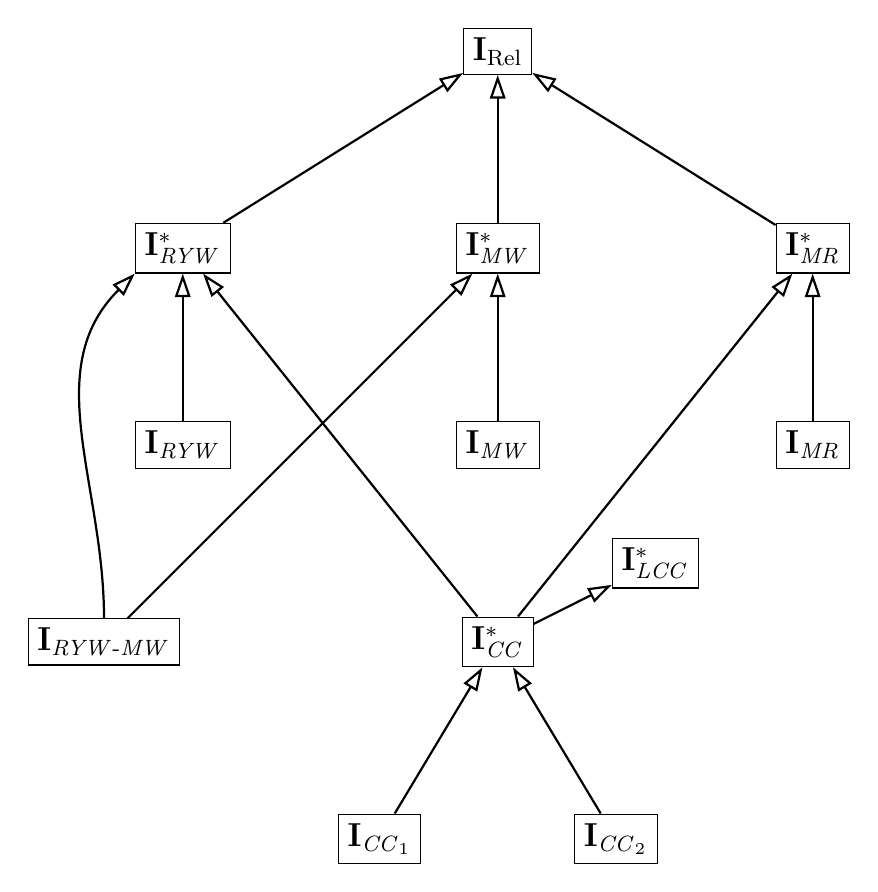
\begin{tikzpicture}[
    every node/.style={font=\large},
    arr/.style={-{Triangle[open, length=3mm]}, thick},
  ]

  % ── Nodes ────────────────────────────────────────────────────────────────

  % Bottom level
  \node[draw] (CC1)    at (-1.5, 0)  {$\mathbf{I}_{\CC_1}$};
  \node[draw] (CC2)    at ( 1.5, 0)  {$\mathbf{I}_{\CC_2}$};

  % Level 1
  \node[draw] (RYWMW)  at (-5,  2.5) {$\mathbf{I}_{\RYW\text{-}\MW}$};
  \node[draw] (CCstar) at ( 0,  2.5) {$\mathbf{I}_{\CC}^{*}$};

  % Level 2 (non-starred)
  \node[draw] (RYW)    at (-4, 5)    {$\mathbf{I}_{\RYW}$};
  \node[draw] (MW)     at ( 0, 5)    {$\mathbf{I}_{\MW}$};
  \node[draw] (MR)     at ( 4, 5)    {$\mathbf{I}_{\MR}$};
  \node[draw] (LCCstar) at ( 2, 3.5)   {$\mathbf{I}_{\LCC}^{*}$};

  % Level 3 (starred)
  \node[draw] (RYWstar) at (-4, 7.5) {$\mathbf{I}_{\RYW}^{*}$};
  \node[draw] (MWstar)  at ( 0, 7.5) {$\mathbf{I}_{\MW}^{*}$};
  \node[draw] (MRstar)  at ( 4, 7.5) {$\mathbf{I}_{\MR}^{*}$};

  % Level 4 (top)
  \node[draw] (Rel)     at ( 0, 10)  {$\mathbf{I}_{\mathrm{Rel}}$};

  % ── Edges ────────────────────────────────────────────────────────────────

  % CC1, CC2 → CC*
  \draw[arr] (CC1)     -- (CCstar);
  \draw[arr] (CC2)     -- (CCstar);

  % RYW-MW → RYW* (routed left of RYW to avoid overlap)
  \draw[arr] (RYWMW.north) to[out=90, in=225] (RYWstar.south west);

  % RYW-MW → MW*
  \draw[arr] (RYWMW)   -- (MWstar);

  % CC* → RYW*, MR*, LCC*
  \draw[arr] (CCstar)  -- (RYWstar);
  \draw[arr] (CCstar)  -- (MRstar);
  \draw[arr] (CCstar)  -- (LCCstar);

  % RYW → RYW*,  MW → MW*,  MR → MR*
  \draw[arr] (RYW)     -- (RYWstar);
  \draw[arr] (MW)      -- (MWstar);
  \draw[arr] (MR)      -- (MRstar);

  % RYW*, MW*, MR* → Rel
  \draw[arr] (RYWstar) -- (Rel);
  \draw[arr] (MWstar)  -- (Rel);
  \draw[arr] (MRstar)  -- (Rel);

  \end{tikzpicture}

  \vspace{0.5em}
  {\small
  \begin{tabular}{@{}ll@{}}
    $\mathbf{I}_{\mathrm{Rel}}$        & Relaxed Specification (Fig.~\ref{fig:relaxed-specification}) \\
    $\mathbf{I}_{\RYW}^{*}$           & Read Your Writes Specification (Fig.~\ref{fig:read-your-writes-spec}) \\
    $\mathbf{I}_{\RYW}$               & Read Your Writes Implementation (Fig.~\ref{fig:read-your-writes-impl}) \\
    $\mathbf{I}_{\MR}^{*}$            & Monotonic Reads Specification (Fig.~\ref{fig:monotonic-reads-spec}) \\
    $\mathbf{I}_{\MR}$                & Monotonic Reads Implementation (Fig.~\ref{fig:monotonic-reads-impl}) \\
    $\mathbf{I}_{\MW}^{*}$            & Monotonic Writes Specification (Fig.~\ref{fig:monotonic-writes-spec}) \\
    $\mathbf{I}_{\MW}$                & Monotonic Writes Implementation (Fig.~\ref{fig:monotonic-writes-impl}) \\
    $\mathbf{I}_{\RYW\text{-}\MW}$    & Read Your Writes and Monotonic Writes Implementation (Fig.~\ref{fig:ryw-mw-impl}) \\
    $\mathbf{I}_{\LCC}^{*}$           & Labeled Causal Consistency Spec (Fig.~\ref{fig:lcc-spec}) \\
    $\mathbf{I}_{\CC}^{*}$            & Causal Consistency Spec (Fig.~\ref{fig:causal-cons-spec}) \\
    $\mathbf{I}_{\CC_1}$              & Causal Consistency Implementation 1 (Fig.~\ref{fig:causal-map-95}) \\
    $\mathbf{I}_{\CC_2}$              & Causal Consistency Implementation 2 (Fig.~\ref{fig:LloydFreedman-protocol}) \\
  \end{tabular}
  }

  \caption{Refinement Hierarchy}
  \label{fig:refinement-hierarchy}
\end{figure}


\clearpage
\begin{figure}
\centering
\specfig{%
\begin{minipage}{0.90\linewidth}
   \figurealgtextsize
   \setlength{\abovedisplayskip}{0pt}%
   \setlength{\abovedisplayshortskip}{0pt}%
   \setlength{\belowdisplayskip}{0pt}%
   \setlength{\belowdisplayshortskip}{0pt}%
   \begin{mathpar}
   \begin{array}{|lr|}
      \hline
         𝐈_{\Rel} \ (\name{Relaxed Specification})
      & \\ \hline
         \CState ≔ \Unit
         & \bnote{Client State}
      \\
         \cInit(c) ≔ ⊥
         & \bnote{Client Initial State}
      \\
         \RState ≔ K ↦ V
         & \bnote{Replica State}
      \\
         \rInit(r, v₀) ≔ [\overline{ k ↦ v₀}]
         & \bnote{Replica Initial State}
      \\
      & \\
         \GetReqPayload ≔ \GetResPayload ≔ \Unit
         & \note{Get payload types}
      \\
         \getReq \ (\_) (\_, σ)  ≔ 
         & \note{At client: } \bnote{Get Request}
      \\ \t
         \ret〈○, p〉
         & \note{No payload}
      \\
         \getGuard \ (\_) (\_) (\_, \_, \_) ≔
         & \note{At replica: } \bnote{Get Guard}
      \\ \t
         \ret \true
         & \note{}
      \\
         \get \ (k) (\_) (\_, \_, ς)  ≔
         & \note{At replica: } \bnote{Get}
      \\ \t
         \llet〈v, \_〉← ς (k)
         & \note{}
      \\ \t
         \ret〈 v, ○, ς 〉
         & \note{No payload}
      \\
         \getRes \ (\_, \_) (\_) (\_, σ) ≔
         & \note{At client: } \bnote{Get Response}
      \\ \t
         \ret σ
         & \note{}
      \\
      & \\
         \PutReqPayload ≔ \Unit
         & \note{Put payload types} 
      \\
         \putReq \ (k, \_) (\_, σ) ≔ 
         & \note{At client: }\bnote{Put Request}
      \\ \t
         \ret〈○, σ〉
         & \note{No payload}
      \\
         \putGuard \ (\_, \_) (\_) (\_, \_, \_) ≔ 
         & \note{At replica: } \bnote{Put Guard}
      \\ \t
         \ret \true
         & \note{}          
      \\
         \lput \ (k, v) (\_) (\_, \_, ς) ≔ 
         & \note{At replica: } \bnote{Put}
      \\ \t
         \ret ς [k ↦ v]
      & \\ \hline
   \end{array}
   \end{mathpar}
\end{minipage}%
}
   \caption{Relaxed Specification}
   \label{fig:relaxed-specification}
\end{figure}


\subsection{Read-Your-Writes (RYW)}
A client's read sees its own most recent write. The session tracks every put the client has issued; the get-guard requires the responding replica to have applied every put in that set (\cref{fig:read-your-writes-spec}). The reference implementation stores per-replica state as a function from key to timestamp (\cref{fig:read-your-writes-impl}).


\clearpage
\begin{figure}
   \figurealgtextsize
   \setlength{\abovedisplayskip}{0pt}%
   \setlength{\abovedisplayshortskip}{0pt}%
   \setlength{\belowdisplayskip}{0pt}%
   \setlength{\belowdisplayshortskip}{0pt}%
   \begin{mathpar}
   \begin{array}{|lr|}
      \hline
         𝐈_{\RYW} ⃰  \ (\name{Read Your Writes Specification}) 
      & \\ \hline
         T ≔ \Nat
         & \note{Timestamp}
      \\
         \CState ≔ 
         & \bnote{Client State}
      \\ \t
%          \Set[C × T × K]
%          & \note{Session puts. ($C × T$ uniquely identifies puts.)}
         \Set[K × T]
         & \note{Session puts. ($T$ uniquely identifies puts in a client.)}
      \\
         \cInit(c) ≔
         & \bnote{Client Initial State}
      \\ \t
         ∅
%          \lif (c = c₀) \
%            \{ 〈c₀, 1〉\} \ 
%          \lelse ∅
         & \note{No initial puts}
      \\
         \RState ≔
         & \bnote{Replica State}
      \\ \t
%          K ↦ (C × T × V × \Set[C × T × K])
         K ↦ (V × C × T \, × 
         & \note{Map from each key $k$ to its value $v$, its origin $〈c, t〉$,}
      \\ \t \phantom{K ↦ (}
%          \Set[C × T])
         \Set[T])
         & \note{and timestamps of puts on $k$ before it.}
      \\
         \rInit(r, v₀) ≔ 
         & \bnote{Replica Initial State}
      \\ \t
         [\overline{ k ↦ 〈v₀, c₀, 0, ∅〉}]
%          [\overline{ k ↦ 〈v₀, c₀, 1, ∅〉}]
         & \note{}
      \\
      & \\
%          \GetReqPayload ≔ \Set[C × T × K]
%          \GetReqPayload ≔ \Set[C × T]
         \GetReqPayload ≔ \Set[T]
         & \note{Get payload types}
      \\
         \GetResPayload ≔ \Unit
      & \\
         \getReq \ (k) (\_, p)  ≔ 
         & \note{At client: } \bnote{Get Request}
      \\ \t
         \ret〈p|ₖ, p〉
         & \note{Session past puts as request payload, State unchanged}
      \\
         \getGuard \ (k)(p)(c, \_, ς) ≔
         & \note{At replica: } \bnote{Get Guard}
      \\ \t
         \llet〈\_, c', t', p'〉← ς (k)
      & \\ \t
%          \ret c = c' ⇒ ¬ (p'|ₖ ∪ \{〈c', t'〉\} ⊂ p|ₖ )
%          \ret c' = c ⇒ ¬ (p' ∪ \{〈c', t'〉\} ⊂ p )
%          \ret c = c' ⇒ p = p' ∪ \{〈c', t'〉\}
%          \ret c = c' ⇒ p ⊆ p' ∪ \{〈c', t'〉\}
         \ret c = c' ⇒ p ⊆ p' ∪ \{ t'\}
%          \ret p|ₖ ⊆ (p'|ₖ ∪ \{〈c', t', k〉\})         
         & \note{If stored value is from requesting client, his puts not missed.}
%          
%       & \\ \t
%          \ret 
%             \lforall (λ〈c ⃰, t ⃰, k ⃰〉. \
%             & \note{If the session puts $d$}
%       \\ \t\t \phantom{\ret \lforall (}
%             k ⃰ = k  ⇒ 
%             & \note{includes any put $〈c ⃰, t ⃰〉$,}
%       \\ \t\t\t \phantom{\ret \lforall (}
%             t ⃰ = 0 ∨〈c ⃰, t ⃰〉= 〈c', t'〉\ ∨
%             & \note{then the current entry for $k$ is $〈c ⃰, t ⃰〉$, or}
%       \\ \t\t\t \phantom{\ret \lforall (}
%             〈c ⃰, t ⃰, k ⃰〉∈ p') \
%             & \note{$〈c ⃰, t ⃰〉$ is in the past puts of the current entry.}
%       \\ \t \phantom{\ret \lforall}
%             p
%          & \note{}
      \\
         \get \ (k) (\_) (\_, \_, ς)  ≔
         & \note{At replica: } \bnote{Get}
      \\ \t
         \llet〈v, \_, \_, \_〉← ς (k)
         & \note{}
      \\ \t
         \ret〈 v, ○, ς 〉
         & \note{No payload}
      \\
         \getRes \ (\_, \_) (\_) (\_, p) ≔
         & \note{At client: } \bnote{Get Response}
      \\ \t
         \ret p
         & \note{State unchanged.}
      \\
      & \\
%          \PutReqPayload ≔ T × \Set[C × T]
         \PutReqPayload ≔ T × \Set[T]
         & \note{Put payload types}
      \\
         \putReq \ (k, \_) (\self, p) ≔ 
         & \note{At client: }\bnote{Put Request}
      \\ \t
         \llet t ← |p| + 1
         & \note{Current put timestamp}
      \\ \t
%          \llet p' ← p ∪ \{〈\self, t, k〉\}
         \llet p' ← p ∪ \{〈t, k〉\}
         & \note{The put is added to session puts.}
      \\ \t
%          \ret〈d|ₖ, d'〉
         \ret〈〈t, p|ₖ〉, p'〉
         & \note{Session puts are sent as request payload.}
      \\
         \putGuard \ (\_, \_) (\_) (\_, \_, \_) ≔ 
         & \note{At replica: } \bnote{Put Guard}
      \\ \t
         \ret \true
         & \note{}          
      \\
         \lput \ (k, v) (〈t, p〉) (c, \_, ς) ≔ 
         & \note{At replica: } \bnote{Put}
      \\ \t
         \ret ς [k ↦ 〈v, c, t, p〉]
      & \\
      & \\
      p|ₖ ≔ \{ t \ | \ 〈t, k〉∈ p \}
      & \\ \hline
   \end{array}
   \end{mathpar}
   \caption{Read Your Writes Specification}
   \label{fig:read-your-writes-spec}
\end{figure}


\clearpage
\begin{figure}
   \figurealgtextsize
   \setlength{\abovedisplayskip}{0pt}%
   \setlength{\abovedisplayshortskip}{0pt}%
   \setlength{\belowdisplayskip}{0pt}%
   \setlength{\belowdisplayshortskip}{0pt}%
   \begin{mathpar}
   \begin{array}{|lr|}
      \hline
         𝐈_{\RYW} \ (\name{Read Your Writes Implementation}) 
      & \\ \hline
         T ≔ \Nat
         & \note{Timestamp}
      \\
         \CState ≔ 
         & \bnote{Client State}
      \\ \t
         K ↦ T
         & \note{Latest put for each key. ($T$ uniquely identifies puts in a client.)}
      \\
         \cInit(c) ≔
         & \bnote{Client Initial State}
      \\ \t
         [ \overline{k ↦ 0} ]
         & \note{No initial puts}
      \\
         \RState ≔
         & \bnote{Replica State}
      \\ \t
         K ↦ (V × C × T) 
         & \note{Map from each key $k$ to its value $v$, and its origin $〈c, t〉$}
      \\
         \rInit(r, v₀) ≔ 
         & \bnote{Replica Initial State}
      \\ \t
         [\overline{ k ↦ 〈v₀, c₀, 0〉}]
         & \note{}
      \\
      & \\
         \GetReqPayload ≔ T
         & \note{Get payload types}
      \\
         \GetResPayload ≔ \Unit
      & \\
         \getReq \ (k) (\_, p)  ≔ 
         & \note{At client: } \bnote{Get Request}
      \\ \t
         \ret〈p(k), p〉
         & \note{Timestamp of latest put as request payload, State unchanged}
      \\
         \getGuard \ (k)(t)(c, \_, ς) ≔
         & \note{At replica: } \bnote{Get Guard}
      \\ \t
         \llet〈\_, c', t'〉← ς (k)
      & \\ \t
         \ret  c = c'  ⇒  t = t' 
%          t ≤ t'
         & \note{If stored value is from requesting client, his puts not missed.}
      \\
         \get \ (k) (\_) (\_, \_, ς)  ≔
         & \note{At replica: } \bnote{Get}
      \\ \t
         \llet〈v, \_, \_〉← ς (k)
         & \note{}
      \\ \t
         \ret〈 v, ○, ς 〉
         & \note{No payload}
      \\
         \getRes \ (\_, \_) (\_) (\_, p) ≔
         & \note{At client: } \bnote{Get Response}
      \\ \t
         \ret p
         & \note{State unchanged.}
      \\
      & \\
         \PutReqPayload ≔ T
         & \note{Put payload types}
      \\
         \putReq \ (k, \_) (\self, p) ≔ 
         & \note{At client: }\bnote{Put Request}
      \\ \t
         \llet t ← p(k) + 1
         & \note{Current put timestamp}
      \\ \t
         \llet p' ← p [ k ↦ t ]
         & \note{The put timestamp is stored as the latest for the key.}
      \\ \t
         \ret〈t, p'〉
         & \note{Latest put timestamp sent as request payload.}
      \\
         \putGuard \ (\_, \_) (\_) (\_, \_, \_) ≔ 
         & \note{At replica: } \bnote{Put Guard}
      \\ \t
         \ret \true
         & \note{}          
      \\
         \lput \ (k, v) (t) (c, \_, ς) ≔
         & \note{At replica: } \bnote{Put}
      \\ \t
         \ret ς [k ↦ 〈v, c, t〉]
      & \\ \hline
   \end{array}
   \end{mathpar}
   \caption{Read Your Writes Implementation}
   \label{fig:read-your-writes-impl}
\end{figure}


\subsection{Monotonic Reads (MR)}
A client's reads respect the order of writes the client has previously observed. The session keeps the set of writes seen so far; subsequent reads must return values applied no earlier than every write in that set (\cref{fig:monotonic-reads-spec}). The reference implementation stores per-replica state as a function from key to (value, client, timestamp); the get-guard checks every entry against the client's session set on every read (\cref{fig:monotonic-reads-impl}).

\clearpage
\begin{figure}
   \figurealgtextsize
   \setlength{\abovedisplayskip}{0pt}%
   \setlength{\abovedisplayshortskip}{0pt}%
   \setlength{\belowdisplayskip}{0pt}%
   \setlength{\belowdisplayshortskip}{0pt}%
   \begin{mathpar}
   \begin{array}{|lr|}
      \hline
         𝐈_{\MR} ⃰  \ (\name{Monotonic Reads Specification})
      & \\ \hline
         T ≔ \Nat
         & \note{Timestamp}
      \\
         \CState ≔ 
         & \bnote{Client State}
      \\ \t
         \Set[T × K] \, ×
         & \note{Session puts. ($C × T$ uniquely identifies puts.)}
      \\ \t 
         \Set[C × T × K]
         & \note{Session dependencies.}         
      \\
         \cInit(c) ≔
         & \bnote{Client Initial State}
      \\ \t
         ∅
         & \note{No initial dependencies}
      \\
         \RState ≔
         & \bnote{Replica State}
      \\ \t
         K ↦ (V × C × T \, ×
         & \note{Map from each key $K$ to its value $V$, its origin $C × T$}
      \\ \t \phantom{K ↦ (}
%          \Set[C × T])
         \Set[T  × K])
         & \note{and puts before it}
      \\
         \rInit(r, v₀) ≔ 
         & \bnote{Replica Initial State}
      \\ \t
         [\overline{ k ↦ 〈v₀, c₀, 0, ∅〉}]
         & \note{}
      \\
      & \\
%          \GetReqPayload ≔ \Set[C × T × K]
%          \GetReqPayload, \GetResPayload ≔ \Set[C × T]
%          \GetReqPayload, \GetResPayload ≔ \Set[C × T]
         \GetReqPayload ≔ \Set[C × T]
         & \note{Get payload types}
      \\
         \GetResPayload ≔ C × T
         & \note{}
      \\
         \getReq \ (k) (\_, 〈p, d〉)  ≔ 
         & \note{At client: } \bnote{Get Request}
      \\ \t
         \ret〈d|ₖ, 〈p, d〉〉
         & \note{Session deps for $k$ sent as payload, State unchanged}
      \\
         \getGuard \ (k) (d) (c, \_, ς) ≔
         & \note{At replica: } \bnote{Get Guard}
      \\ \t
         \llet〈\_, c', t', d'〉← ς (k)
      & \\ \t
%          \ret d|_{c'} ⊆ d' ∪ \{〈c', t'〉\}
         \ret d|_{c'} ⊆ d'|ₖ ∪ \{ t' \}
%          & \note{Observed puts from $c'$ are not after stored put from $c'$.}
         & \note{Stored put from $c'$ doesn't miss observed puts from $c'$.}
      \\
         \get \ (k) (\_) (\_, \_, ς)  ≔
         & \note{}
      \\ \t
         \llet〈v, c, t, d〉← ς (k)
      & \\ \t
         \ret〈 v, 〈c, t〉, ς 〉
         & \note{The stored put returned as a dependency.}
      \\
         \getRes \ (k, \_) (〈c, t〉) (\_, 〈p, d〉) ≔
         & \note{At client: } \bnote{Get Response}
      \\ \t
%          \ret d ∪ (c ▹ d' ▹ k)
         \ret 〈p, d ∪ \{ 〈c, t, k〉\}〉
%          \ret d ∪ d'
%          \ret d ∪ (c ▹ d')
%          \ret d ∪ (\lmap (λ〈t, k〉. \ 〈c, t, k〉) \ d'
         & \note{Returned dependency added to session dependencies.}
      \\
      & \\
         \PutReqPayload ≔ T × \Set[T × K]
         & \note{Put payload types}
      \\
         \putReq \ (k, \_) (\_, 〈p, d〉) ≔ 
         & \note{At client: }\bnote{Put Request}
      \\ \t
%          \llet t ← |\{〈c, \_, \_〉∈ p \ | \ c=\self \}| + 1
%          \llet t ← | \, d|_\self \, | + 1
         \llet t ← | p | + 1
         & \note{Current put timestamp}
      \\ \t
         \llet p' ← p ∪ \{〈t, k〉\}
         & \note{The put is added to session puts.}
      \\ \t
%          \ret〈〈t, d|ₖ|ₚ〉, d'〉
%          \ret〈〈t, d|_{\self}|ₖ〉, d'〉
         \ret〈〈t, p〉, 〈p', d〉〉
         & \note{Session puts are sent as request payload.}
      \\
         \putGuard \ (\_, \_) (\_) (\_, \_, \_) ≔ 
         & \note{At replica: } \bnote{Put Guard}
      \\ \t
         \ret \true
         & \note{}          
      \\
         \lput \ (k, v) (〈t, p〉) (c, \_, ς) ≔ 
         & \note{At replica: } \bnote{Put}
      \\ \t
         \ret ς [k ↦ 〈v, c, t, p〉]
      & \\
      & \\
      d|ₖ ≔ \{〈c, t〉 \ | \ 〈c, t, k〉∈ d \}
      & \\
      d|ₖ ≔ \{ t \ | \ 〈t, k〉∈ d \}
%       & \\
%       d|_c  ≔ \{〈t, k〉 \ | \ 〈c, t, k〉∈ d \}
      & \\
      d|_c  ≔ \{ t \ | \ 〈c, t〉∈ d \}
%       & \\
%       c ▹ d ≔ \lmap (λ〈t, k〉. \ 〈c, t, k〉) \ d
      & \\ \hline
   \end{array}
   \end{mathpar}
   \caption{Monotonic Reads Specification}
   \label{fig:monotonic-reads-spec}
\end{figure}

\clearpage
\begin{figure}
   \figurealgtextsize
   \setlength{\abovedisplayskip}{0pt}%
   \setlength{\abovedisplayshortskip}{0pt}%
   \setlength{\belowdisplayskip}{0pt}%
   \setlength{\belowdisplayshortskip}{0pt}%
   \begin{mathpar}
   \begin{array}{|lr|}
      \hline
         𝐈_{\MR} \ (\name{Monotonic Reads Implementation})
      & \\ \hline
         T ≔ \Nat
         & \note{Timestamp}
      \\
         \CState ≔ 
         & \bnote{Client State}
      \\ \t
         T \ ×
         & \note{Session latest put timestamp}
      \\ \t
         K ↦ C ↦ T
         & \note{Largest timestamp read for the key from the client.}         
      \\
         \cInit(c) ≔
         & \bnote{Client Initial State}
      \\ \t
         〈∅, ∅〉
         & \note{No initial puts and dependencies}
      \\
         \RState ≔
         & \bnote{Replica State}
      \\ \t
         K ↦ (V × C × T)
         & \note{Map from each key $K$ to its value $V$, its origin $C × T$}
%       \\ \t \phantom{K ↦ (}
% %          \Set[C × T])
%          K ↦ T)
%          & \note{and puts before it}
      \\
         \rInit(r, v₀) ≔ 
         & \bnote{Replica Initial State}
      \\ \t
         [\overline{ k ↦ 〈v₀, c₀, 0〉}]
         & \note{}
      \\
      & \\
         \GetReqPayload ≔ \Set[C × T]
         & \note{Get payload types}
      \\
         \GetResPayload ≔ C × T
         & \note{}
      \\
         \getReq \ (k) (\_, 〈t, d〉)  ≔ 
         & \note{At client: } \bnote{Get Request}
      \\ \t
         \ret〈d(k), 〈t, d〉〉
         & \note{Session deps for $k$ sent as payload, State unchanged}
      \\
         \getGuard \ (k) (d) (c, \_, ς) ≔
         & \note{At replica: } \bnote{Get Guard}
      \\ \t
         \llet〈\_, c', t'〉← ς (k)
      & \\ \t
         \ret d(c') ≤  t'
         & \note{Stored put from $c'$ doesn't miss observed puts from $c'$.}
      \\
         \get \ (k) (\_) (\_, \_, ς)  ≔
         & \note{}
      \\ \t
         \llet〈v, c, t〉← ς (k)
      & \\ \t
         \ret〈 v, 〈c, t〉, ς 〉
         & \note{The stored put returned as a dependency.}
      \\
         \getRes \ (k, \_) (〈c, t〉) (\_, 〈t, d〉) ≔
         & \note{At client: } \bnote{Get Response}
      \\ \t
         \ret〈t, d[〈k,c〉 ↦ t] 〉
         & \note{Returned dependency advances session dependencies.}
      \\
      & \\
         \PutReqPayload ≔ T
         & \note{Put payload types}
      \\
         \putReq \ (k, \_) (\_, 〈t, d〉) ≔ 
         & \note{At client: }\bnote{Put Request}
      \\ \t
         \llet t' ← t + 1
         & \note{Current put timestamp}
      \\ \t
         \ret〈t', 〈t', d〉〉
         & \note{}
      \\
         \putGuard \ (\_, \_) (\_) (\_, \_, \_) ≔ 
         & \note{At replica: } \bnote{Put Guard}
      \\ \t
         \ret \true
         & \note{}          
      \\
         \lput \ (k, v) (t) (c, \_, ς) ≔ 
         & \note{At replica: } \bnote{Put}
      \\ \t
         \ret ς [k ↦ 〈v, c, t〉]
      & \\ \hline
   \end{array}
   \end{mathpar}
   \caption{Monotonic Reads Implementation}
   \label{fig:monotonic-reads-impl}
\end{figure}


\subsection{Monotonic Writes (MW)}
A single client's writes are observed in order at every replica that observes them. Each replica records, per writing client, the latest applied timestamp; the put-guard rejects any out-of-order delivery (\cref{fig:monotonic-writes-spec}). The reference implementation prepends the timestamp of each new write to a per-key list with no de-duplication, so receivers can re-check ordering on every delivery (\cref{fig:monotonic-writes-impl}).


\clearpage
\begin{figure}
   \figurealgtextsize
   \setlength{\abovedisplayskip}{0pt}%
   \setlength{\abovedisplayshortskip}{0pt}%
   \setlength{\belowdisplayskip}{0pt}%
   \setlength{\belowdisplayshortskip}{0pt}%
   \begin{mathpar}
   \begin{array}{|lr|}
      \hline
         𝐈_{\MW} ⃰  \ (\name{Monotonic Writes Specification}) 
      & \\ \hline
         T ≔ \Nat
         & \note{Timestamp}
      \\
         \CState ≔ 
         & \bnote{Client State}
      \\ \t
         \Set[T × K]
         & \note{Session puts. ($C × T$ uniquely identifies puts.)}
      \\
         \cInit(c) ≔
         & \bnote{Client Initial State}
      \\ \t
         ∅
         & \note{No initial dependencies}
      \\
         \RState ≔
         & \bnote{Replica State}
      \\ \t
         K ↦ (V × \Set[C × T])
         & \note{Map from each key $K$ to its value $V$, and puts already applied.}
      \\
         \rInit(r, v₀) ≔ 
         & \bnote{Replica Initial State}
      \\ \t
         [\overline{ k ↦ 〈v₀, ∅〉}]
         & \note{}
      \\
      & \\
         \GetReqPayload ≔ \GetResPayload ≔ \Unit
         & \note{Get payload types}
      \\
         \getReq \ (\_) (\_, p)  ≔ 
         & \note{At client: } \bnote{Get Request}
      \\ \t
         \ret〈○, p〉
         & \note{Session past puts as request payload, State unchanged}
      \\
         \getGuard \ (\_) (\_) (\_, \_, \_) ≔
         & \note{At replica: } \bnote{Get Guard}
      \\ \t
         \ret \true
         & \note{}
      \\
         \get \ (k) (\_) (\_, \_, ς)  ≔
         & \note{At replica: } \bnote{Get}
      \\ \t
         \llet〈v, \_〉← ς (k)
         & \note{}
      \\ \t
         \ret〈 v, ○, ς 〉
         & \note{No payload}
      \\
         \getRes \ (\_, \_) (\_) (\_, p) ≔
         & \note{At client: } \bnote{Get Response}
      \\ \t
         \ret p
         & \note{State unchanged.}
      \\
      & \\
         \PutReqPayload ≔ T × \Set[T]
         & \note{Put payload types}
      \\
         \putReq \ (k, \_) (\_, p) ≔ 
         & \note{At client: }\bnote{Put Request}
      \\ \t
         \llet t ← |p| + 1
         & \note{Current put timestamp}
      \\ \t
         \llet p' ← p ∪ \{〈t, k〉\}         
         & \note{The put is added to session puts.}
      \\ \t
         \ret〈〈t, p|ₖ〉, p'〉
         & \note{Session puts for the key are sent as request payload.}
      \\
         \putGuard \ (k, \_) (〈t, p〉) (c, \_, ς) ≔ 
         & \note{At replica: } \bnote{Put Guard}
      \\ \t
         \llet〈\_, p'〉← ς (k)
      & \\ \t
         \ret p ⊆ p'|_c
         & \note{Previous puts of session already applied.}
      \\
         \lput \ (k, v) (〈t, \_〉) (c, \_, ς) ≔ 
         & \note{At replica: } \bnote{Put}
      \\ \t
         \llet〈\_, p'〉← ς (k)
         & \note{}
      \\ \t
         \ret ς [k ↦ 〈v, p' ∪ \{〈c,t〉\}]
      & \\
      & \\
      p|ₖ ≔ \{ t \ | \ 〈t, k〉∈ p \}
      & \\
      p|_c  ≔ \{ t \ | \ 〈c, t〉∈ p \}
      & \\ \hline
   \end{array}
   \end{mathpar}
   \caption{Monotonic Writes Specification}
   \label{fig:monotonic-writes-spec}
\end{figure}


\clearpage
\begin{figure}
   \figurealgtextsize
   \setlength{\abovedisplayskip}{0pt}%
   \setlength{\abovedisplayshortskip}{0pt}%
   \setlength{\belowdisplayskip}{0pt}%
   \setlength{\belowdisplayshortskip}{0pt}%
   \begin{mathpar}
   \begin{array}{|lr|}
      \hline
         𝐈_{\MW} \ (\name{Monotonic Writes Implementation}) 
      & \\ \hline
         T ≔ \Nat
         & \note{Timestamp}
      \\
         \CState ≔ 
         & \bnote{Client State}
%       \\ \t
%          T \ ×
%          & \note{Latest timestamp, and}
      \\ \t         
         K ↦ T
         & \note{Latest timestamp of puts for the key.}
      \\
         \cInit(c) ≔
         & \bnote{Client Initial State}
      \\ \t
%          〈0, \overline{k ↦ 0}〉
         \overline{k ↦ 0}
         & \note{No initial puts}
      \\
         \RState ≔
         & \bnote{Replica State}
      \\ \t
         K ↦ (V \ ×
         & \note{Map from each key $K$ to its value $V$, and}
      \\ \t \phantom{K ↦ (}
         C ↦ T)
         & \note{latest puts applied from sessions.}
      \\
         \rInit(r, v₀) ≔ 
         & \bnote{Replica Initial State}
      \\ \t
         [\overline{ k ↦ 〈v₀, \overline{c ↦ 0}〉}]
         & \note{}
      \\
      & \\
         \GetReqPayload ≔ \GetResPayload ≔ \Unit
         & \note{Get payload types}
      \\
         \getReq \ (\_) (\_, σ)  ≔ 
         & \note{At client: } \bnote{Get Request}
      \\ \t
         \ret〈○, σ〉
         & \note{Session past puts as request payload, State unchanged}
      \\
         \getGuard \ (\_) (\_) (\_, \_, \_) ≔
         & \note{At replica: } \bnote{Get Guard}
      \\ \t
         \ret \true
         & \note{}
      \\
         \get \ (k) (\_) (\_, \_, ς)  ≔
         & \note{At replica: } \bnote{Get}
      \\ \t
         \llet〈v, \_〉← ς (k)
         & \note{}
      \\ \t
         \ret〈 v, ○, ς 〉
         & \note{No payload}
      \\
         \getRes \ (\_, \_) (\_) (\_, σ) ≔
         & \note{At client: } \bnote{Get Response}
      \\ \t
         \ret σ
         & \note{State unchanged.}
      \\
      & \\
         \PutReqPayload ≔ T
         & \note{Put payload types}
      \\
         \putReq \ (k, \_) (\_, p) ≔ 
         & \note{At client: }\bnote{Put Request}
      \\ \t
         t ← p(k)
         & \note{}
      \\ \t
         \llet p' ← p [ k ↦ t + 1]
         & \note{The timestamp of the latest put for key is advanced.}
      \\ \t
         \ret〈t, p'〉
         & \note{Latest put timestamp for the key is sent as request payload.}
      \\
         \putGuard \ (k, \_) (t) (c, \_, ς) ≔ 
         & \note{At replica: } \bnote{Put Guard}
      \\ \t
         \llet〈\_, p'〉← ς (k)
      & \\ \t
         \ret  p'(c) = t
         & \note{Previous puts of session already applied.}
      \\
         \lput \ (k, v) (t) (c, \_, ς) ≔ 
         & \note{At replica: } \bnote{Put}
      \\ \t
         \llet〈\_, p'〉← ς (k)
         & \note{}
      \\ \t
         \ret ς [k ↦ 〈v, p' [c ↦ t + 1]〉]
         & \note{}
      \\ \hline
   \end{array}
   \end{mathpar}
   \caption{Monotonic Writes Implementation}
   \label{fig:monotonic-writes-impl}
\end{figure}


\subsection{Read-Your-Writes $+$ Monotonic Writes (RYW+MW)}
Composition of Read-Your-Writes and Monotonic Writes. RYW+MW is the conjunction of RYW and MW rather than an independent property; an implementation satisfies it iff it refines both, so correctness is the joint refinement obligation. The reference combines RYW's read-side check with MW's compare-and-swap on every put (\cref{fig:ryw-mw-impl}).

\clearpage
\begin{figure}
   \figurealgtextsize
   \setlength{\abovedisplayskip}{0pt}%
   \setlength{\abovedisplayshortskip}{0pt}%
   \setlength{\belowdisplayskip}{0pt}%
   \setlength{\belowdisplayshortskip}{0pt}%
   \begin{mathpar}
   \begin{array}{|lr|}
      \hline
         \multicolumn{2}{|l|}{𝐈_{\RYW\text{-}\MW} \ (\name{Read Your Writes and Monotonic Writes Implementation}) }         
      \\ \hline
         T ≔ \Nat
         & \note{Timestamp}
      \\
         \CState ≔ 
         & \bnote{Client State}
      \\ \t         
         K ↦ T
         & \note{Latest timestamp of puts for the key.}
      \\
         \cInit(c) ≔
         & \bnote{Client Initial State}
      \\ \t
         \overline{k ↦ 0}
         & \note{No initial puts}
      \\
         \RState ≔
         & \bnote{Replica State}
      \\ \t
         K ↦ (V × C \ × 
         & \note{Map from each key $K$ to its value $V$, and its originating sessions $C$,}
      \\ \t \phantom{K ↦ (}
         C ↦ T)
         & \note{latest puts applied from sessions}
      \\
         \rInit(r, v₀) ≔ 
         & \bnote{Replica Initial State}
      \\ \t
         [\overline{ k ↦ 〈v₀, 0, \overline{c ↦ 0}〉}]
         & \note{}
      \\
      & \\
         \GetReqPayload ≔ T
         & \note{Get payload types}
      \\
         \GetResPayload ≔ \Unit
      & \\
         \getReq \ (k) (\_, p)  ≔ 
         & \note{At client: } \bnote{Get Request}
      \\ \t
         \ret〈p(k), p〉
         & \note{Timestamp of latest put as request payload, State unchanged}
      \\
         \getGuard \ (k)(t)(c, \_, ς) ≔
         & \note{At replica: } \bnote{Get Guard}
      \\ \t
         \llet〈\_, c', p'〉← ς (k)
      & \\ \t
         \ret  c = c'  ⇒  p'(c') = t
%          t ≤ t'
         & \note{If stored value is from requesting client, his puts not missed.}
      \\
         \get \ (k) (\_) (\_, \_, ς)  ≔
         & \note{At replica: } \bnote{Get}
      \\ \t
         \llet〈v, \_, \_〉← ς (k)
         & \note{}
      \\ \t
         \ret〈 v, ○, ς 〉
         & \note{No payload}
      \\
         \getRes \ (\_, \_) (\_) (\_, p) ≔
         & \note{At client: } \bnote{Get Response}
      \\ \t
         \ret p
         & \note{State unchanged.}
      \\
      & \\
         \PutReqPayload ≔ T
         & \note{Put payload types}
      \\
         \putReq \ (k, \_) (\_, p) ≔ 
         & \note{At client: }\bnote{Put Request}
      \\ \t
         t ← p(k)
         & \note{}
      \\ \t
         \llet p' ← p [ k ↦ t + 1 ]
         & \note{The timestamp of the latest put for key is advanced.}
      \\ \t
         \ret〈t, p'〉
         & \note{Latest put timestamp for the key is sent as request payload.}
      \\
         \putGuard \ (k, \_) (t) (c, \_, ς) ≔ 
         & \note{At replica: } \bnote{Put Guard}
      \\ \t
         \llet〈\_, \_, p'〉← ς (k)
      & \\ \t
         \ret p'(c) = t
         & \note{Previous puts of session already applied.}
      \\
         \lput \ (k, v) (t) (c, \_, ς) ≔ 
         & \note{At replica: } \bnote{Put}
      \\ \t
         \llet〈\_, p'〉← ς (k)
         & \note{}
      \\ \t
         \ret ς [k ↦ 〈v, c, p' [c ↦ t + 1]〉]
         & \note{}
      \\ \hline
   \end{array}
   \end{mathpar}
   \caption{Read Your Writes and Monotonic Writes Implementation}
   \label{fig:ryw-mw-impl}
\end{figure}


\subsection{Causal Consistency (CC) and Labeled Causal Consistency (LCC)}
\textbf{Causal Consistency (CC).}
Cross-client causal consistency: every read returns a value whose causal predecessors have all been observed at the responding replica. Dependencies are tracked as explicit sets in the spec state (\cref{fig:causal-cons-spec}), which the implementation must bridge to its concrete representation (typically a per-client vector clock plus a compare-and-swap on the writer's own slot during put). Two reference implementations are given: a per-client vector-clock store (\cref{fig:causal-map-95}) and a Lloyd--Freedman-style protocol (\cref{fig:LloydFreedman-protocol}).

\noindent\textbf{Labeled Causal Consistency (LCC).}
Causal consistency parameterised by per-message topic labels and per-client interest masks. Every put is tagged with a label, and every client declares which labels it cares about; the get-guard requires the responding replica to have observed every dependency whose label is in the requesting client's mask (\cref{fig:lcc-spec}). To our knowledge this is the first \coq{} formalisation of LCC and the first verified implementation.



\clearpage
\begin{figure}
   \figurealgtextsize
   \setlength{\abovedisplayskip}{0pt}%
   \setlength{\abovedisplayshortskip}{0pt}%
   \setlength{\belowdisplayskip}{0pt}%
   \setlength{\belowdisplayshortskip}{0pt}%
   \begin{mathpar}
   \begin{array}{|lr|}
      \hline
         𝐈_{\CC} ⃰  \ (\name{Causal Consistency Spec}) 
      & \\ \hline
         T ≔ \Nat
         & \note{Timestamp}
      \\
         \CState ≔ 
         & \bnote{Client State}
      \\ \t
         〈\Set[C × T × K],
%          〈K ↦ \Set[C × T],
         & \note{Session dependencies from puts.}
      \\ \t \phantom{〈}
         \Set[\Set[C × T × K]] 〉
%          \Set[C × T]
%          & \note{Put timestamp, and Session dependencies}
%          & \note{Current timestamp, and Session dependencies.}
         & \note{Session dependencies from gets}
      \\ \t
         & \note{($C × T$ uniquely identifies puts.)}         
%       \\ \t
%          & \note{($C × T$ uniquely identifies puts.)}
      \\
         \cInit(c) ≔
         & \bnote{Client Initial State}
      \\ \t
%          〈0, ∅〉
         〈∅, ∅〉
%          \lif (c ≠ c₀) \
%          〈∅, ∅〉\ 
%          \lelse  〈[ \overline{k ↦〈c₀, k + 1〉}], ∅〉
         & \note{No initial dependencies}
      \\
         \RState ≔
         & \bnote{Replica State}
      \\ \t
         K ↦ (V × C × T \, × 
%          K ↦ (C × T × V × \Set [C × T])
         & \note{Map from each key $K$ to its value $V$, its origin $C × T$,}
      \\ \t \phantom{K ↦ (}         
         \Set[C × T × K])
         & \note{and set of dependencies}
      \\
         \rInit(r, v₀) ≔ 
         & \bnote{Replica Initial State}
      \\ \t
         [\overline{ k ↦ 〈v₀, c₀, 0, ∅〉}]
%          [\overline{ k ↦ 〈v₀, c₀, k+1, ∅〉}]
%          & \note{For each key, initial $v₀$ and empty initial dependencies}
         & \note{Empty initial dependencies}
      \\
      & \\
         \GetReqPayload ≔ 〈\Set[C × T × K],
         & \note{Get payload types}
      \\ \phantom{\GetReqPayload ≔ 〈}
         \Set[\Set[C × T × K]]\>
%          \GetReqPayload ≔ \Set[C × T]
         & \note{}
      \\
         \GetResPayload ≔ \Set[C × T  × K]
      & \\
         \getReq \ (k) (\_, 〈p, G〉)  ≔ 
         & \note{At client: } \bnote{Get Request}
      \\ \t
         \ret〈〈p|ₖ, G|ₖ〉, 〈p, G〉〉 
         & \note{Session deps sent as request payload, State unchanged}
      \\
         \getGuard \ (k) (〈p, G〉) (c, \_, ς) ≔
         & \note{At replica: } \bnote{Get Guard}
      \\ \t
         \llet〈\_, c', t', d'〉← ς (k)
         & \note{}
      \\ \t
         \ret \lforall (λ d. \ ¬ (d'|ₖ ∪ \{〈c', t', k〉\} ⊂ d)) \ G \ ∧
         & \note{Stored value isn't behind any previously read value.}
%       & \\ \t
%          \ret ¬ (d'|ₖ ∪ \{〈c', t', k〉\} ⊂ d|ₖ)
%          & \note{The stored value is not behind.}
%       \\ \t
%          \ret d|ₖ  ⊆  d'|ₖ ∪ \{〈c', t', k〉\} ∨〈c', t', k〉∉ d|ₖ
%          & \note{Alternative condition}
      \\ \t \phantom{\ret}
         c = c' ⇒ p ⊆ d'|ₖ ∪ \{〈c', t', k〉\}
%          c = c' ⇒ p ⊆ p' ∪ \{ t' \}
         & \note{Read your writes.}
      \\
         \get \ (k) (\_) (\_, \_, ς)  ≔
         & \note{At replica: } \bnote{Get}
      \\ \t
         \llet〈v, c, t, d〉← ς (k)
      & \\ \t
%          \llet d' ← d ∪ \{〈c, t, k〉\}
         \llet d' ← \lif (c ≠ c₀) \ d ∪ \{〈c, t, k〉\} \ \lelse ∅
         & \note{The dependencies returned to the session}
      \\ \t
         \ret〈 v, d', ς 〉
         & \note{are the entry and its dependencies}
      \\
         \getRes \ (\_, \_) (d') (\_, 〈p, G〉) ≔
%          (C, \CState)(K, V, \GetResPayload) → \Unit
         & \note{At client: } \bnote{Get Response}
%       \\ \t
%          \llet 〈t, d'〉 ← σ
%          & \note{The received dependencies are}
      \\ \t
         \ret 〈p, G ∪ \{ d' \}〉
%          & \note{added to the dependencies of the session.}
         & \note{Received dependencies added to session dependencies.}
%       \\ \t
%          \ret d'
      \\
      & \\
         \PutReqPayload ≔ T × \Set [ C × T × K ]
         & \note{Put payload types}
      \\
         \putReq \ (k, \_) (\self, 〈p, G〉) ≔ 
         & \note{At client: }\bnote{Put Request}
      \\ \t
%          \llet t ← |\{〈c, \_, \_〉∈ p \ | \ c=\self \}| + 1
         \llet t ← |p| + 1
         & \note{Current put timestamp}
      \\ \t
         \llet p' ← p ∪ \{〈 \self, t, k 〉\}
         & \note{The put is added to session dependencies.}
      \\ \t
         \ret〈〈t, p ∪ (⋃\, G)〉, 〈p', G〉〉 
         & \note{Session dependencies are sent as request payload.}
      \\
         \putGuard \ (k, \_) (〈t, \_〉) (c, \_, ς) ≔ 
         & \note{At replica: } \bnote{Put Guard}
%       \\ \t
%       \llet t ← |\{〈c', \_, \_〉∈ d \ | \ c'=c \}| + 1
%          & \note{Current put timestamp}
      \\ \t
         \llet〈\_, \_, \_, d'〉← ς (k)
      & \\ \t
          \ret〈c, t, k〉∉ d'
          & \note{The new put is not causally before the current stored put.}
      \\
         \lput \ (k, v) (〈t, d〉) (c, \_, ς) ≔ 
         & \note{At replica: } \bnote{Put}
%       \\ \t
%       \llet t ← |\{〈c', \_, \_〉∈ d \ | \ c'=c \}| + 1
%          & \note{Current put timestamp}
      \\ \t
         \ret ς [k ↦ 〈v, c, t, d〉]
%          ς' ← ς [k ↦ 〈c, t, v, d〉]
%       & \\ \t
%          \ret ς'
      & \\
      & \\
         d|ₖ ≔ \{〈c, t, k〉\ | \ 〈c, t, k'〉∈ d  ∧ k = k' \}
%          \{〈c', t', k'〉∈ d \ | \ k = k' \}
      & \\
         D|ₖ ≔ \{ d|ₖ \ | \ d ∈ D \}
      & \\ \hline
   \end{array}
   \end{mathpar}
   \caption{Causal Consistency Spec}
   \label{fig:causal-cons-spec}
\end{figure}



\clearpage
\begin{figure}
   \figurealgtextsize
   \setlength{\abovedisplayskip}{0pt}%
   \setlength{\abovedisplayshortskip}{0pt}%
   \setlength{\belowdisplayskip}{0pt}%
   \setlength{\belowdisplayshortskip}{0pt}%
   \begin{mathpar}
   \begin{array}{|lr|}
      \hline
         𝐈_{\LCC} ⃰  \ (\name{Labeled Causal Consistency Spec})
      & \\ \hline
         \L
         & \note{Label type}
      \\
         \lab : V → \L
         & \note{Maps each value to its label}
      \\
         \clientLabs : C → \Set[\L]
         & \note{Maps each client to its set of relevant labels}
      \\
         T ≔ \Nat
         & \note{Timestamp}
      \\
         \CState ≔
         & \bnote{Client State}
      \\ \t
         〈\Set[C × T × K × \L],
         & \note{Session dependencies from puts (with labels)}
      \\ \t \phantom{〈}
         \Set[\Set[C × T × K × \L]] 〉
         & \note{Session dependencies from gets (with labels)}
      \\
         \cInit(c) ≔
         & \bnote{Client Initial State}
      \\ \t
         〈∅, ∅〉
         & \note{No initial dependencies}
      \\
         \RState ≔
         & \bnote{Replica State}
      \\ \t
         K ↦ (V × C × T \, ×
         & \note{Map from each key $K$ to its value $V$, its origin $C × T$,}
      \\ \t \phantom{K ↦ (}
         \Set[C × T × K × \L])
         & \note{and set of label-annotated dependencies}
      \\
         \rInit(r, v₀) ≔
         & \bnote{Replica Initial State}
      \\ \t
         [\overline{ k ↦ 〈v₀, c₀, 0, ∅〉}]
         & \note{Empty initial dependencies}
      \\
      & \\
         \GetReqPayload ≔ 〈\Set[C × T × K × \L]
         & \note{Get payload types}
      \\ \phantom{\GetReqPayload ≔ 〈}
         \Set[\Set[C × T × K × \L]]
      & \\
         \GetResPayload ≔ \Set[C × T × K × \L]
      & \\
         \getReq \ (k) (\self, 〈p, G〉)  ≔
         & \note{At client: } \bnote{Get Request}
      \\ \t
         \llet L ← \clientLabs(\self)
      & \\ \t
         \ret〈〈p|ₖ|_{L}, G|ₖ|_{L}〉, 〈p, G〉〉
         & \note{Label-filtered deps sent as payload; state unchanged.}
      \\
         \getGuard \ (k) (〈p, G〉) (c, \_, ς) ≔
         & \note{At replica: } \bnote{Get Guard}
      \\ \t
         \llet〈v', c', t', d'〉← ς (k)
      & \\ \t
         \llet L ← \clientLabs(c)
      & \\ \t
         \ret \lforall (λ d. \ 
         & \note{Stored value not behind any previously}
      \\ \t \ \ \ \
         ¬ ((d'|ₖ ∪ \{〈c', t', k, \lab(v')〉\})|_{L} ⊂ d)) \ G
         & \note{read value, for client's labels.}
      \\ \t
         ∧ \ c = c' ⇒ p ⊆ d'|ₖ ∪ \{〈c', t', k, \lab(v')〉\}
         & \note{Read your writes.}         
      \\
         \get \ (k) (\_) (\_, \_, ς)  ≔
         & \note{At replica: } \bnote{Get}
      \\ \t
         \llet〈v, c, t, d〉← ς (k)
      & \\ \t
         \llet d' ← \lif (c ≠ c₀) \ d ∪ \{〈c, t, k, \lab(v)〉\} \ \lelse ∅
         & \note{Label of stored value included in returned dependency.}
      \\ \t
         \ret〈 v, d', ς 〉
         & \note{}
      \\
         \getRes \ (\_, \_) (d') (\_, 〈p, G〉) ≔
         & \note{At client: } \bnote{Get Response}
      \\ \t
         \ret 〈p, G ∪ \{ d' \}〉
         & \note{Received dependencies added to session.}
      \\
      & \\
         \PutReqPayload ≔ T × \Set [ C × T × K × \L ]
         & \note{Put payload types}
      \\
         \putReq \ (k, v) (\self, 〈p, G〉) ≔
         & \note{At client: }\bnote{Put Request}
      \\ \t
         \llet t ← |p| + 1
         & \note{Current put timestamp}
      \\ \t
         \llet p' ← p ∪ \{〈 \self, t, k, \lab(v) 〉\}
         & \note{Put with its label added to session dependencies.}
      \\ \t
         \ret〈〈t, p ∪ (⋃\, G)〉, 〈p', G〉〉
         & \note{All session dependencies sent as request payload.}
      \\
         \putGuard \ (k, v) (〈t, \_〉) (c, \_, ς) ≔
         & \note{At replica: } \bnote{Put Guard}
      \\ \t
         \llet〈\_, \_, \_, d'〉← ς (k)
      & \\ \t
          \ret〈c, t, k, \lab(v)〉∉ d'
          & \note{The new put has not already been applied.}
      \\
         \lput \ (k, v) (〈t, d〉) (c, \_, ς) ≔
         & \note{At replica: } \bnote{Put}
      \\ \t
         \ret ς [k ↦ 〈v, c, t, d〉]
      & \\
      & \\
         d|ₖ ≔ \{〈c, t, k, l〉\ | \ 〈c, t, k', l〉∈ d  ∧ k = k' \}
      & \\
         D|ₖ ≔ \{ d|ₖ \ | \ d ∈ D \}
      & \\
         d|_{L} ≔ \{〈c, t, k, l〉\ | \ 〈c, t, k, l〉∈ d  ∧ l ∈ L \}
         & \note{Filter dependencies to the label set $L$}
      \\
         D|_{L} ≔ \{ d|_{L} \ | \ d ∈ D \}
      & \\ \hline
   \end{array}
   \end{mathpar}
   \caption{Labeled Causal Consistency Spec. 
   Causal consistency — but per topic. Every put is tagged with a label (think: Kafka topic, Slack channel, pub/sub subject). Every client declares which labels it cares about. Causal delivery for a client is enforced only for labels the client is interested in.}
   \label{fig:lcc-spec}
\end{figure}


\clearpage
\begin{figure}
   \figurealgtextsize
   \setlength{\abovedisplayskip}{0pt}%
   \setlength{\abovedisplayshortskip}{0pt}%
   \setlength{\belowdisplayskip}{0pt}%
   \setlength{\belowdisplayshortskip}{0pt}%
   \begin{mathpar}
   \begin{array}{|lr|}
      \hline
         \multicolumn{2}{|l|}{𝐈_{\CC_1} \ (\name{Causal Consistency Implementation 1})}
      \\ \hline
         T ≔ \Nat
         & \note{Timestamp}
      \\
         \CState ≔ 
         & \bnote{Client State}
      \\ \t
         C ↦ T
         & \note{Session vector-clock}
      \\
         \cInit(c) ≔
         & \bnote{Client Initial State}
      \\ \t
         [\overline{ c ↦ 0 }]
         & \note{No initial dependencies}
      \\
         \RState ≔
         & \bnote{Replica State}
      \\ \t
         〈K ↦ V, \
%          〈K ↦ C × T × V, \
%          For later C and T stored too
         & \note{Store}  % ($C × T$ uniquely identifies puts.)
      \\ \t \phantom{〈}
          C ↦ T〉          
%          〈K ↦ V , \ C ↦ T〉
%          & \note{Dependencies vector-clock (one for all keys)}
         & \note{Received vector-clock (one for all keys)}
      \\
         \rInit(r, v₀) ≔ 
         & \bnote{Replica Initial State}
      \\ \t
         〈[\overline{ k ↦ v₀}], [\overline{ c ↦ 0 }]〉
%          & \note{For each key, initial $v₀$ and empty initial dependencies}
         & \note{Empty initial dependencies}
      \\
      & \\
         \GetReqPayload ≔ C ↦ T
         & \note{Get payload types}
      \\
         \GetResPayload ≔ C ↦ T
      & \\
         \getReq \ (\_) (\_, d)  ≔ 
         & \note{At client: } \bnote{Get Request}
%       \\ \t
%          \llet d ← σ 
%       & \\ \t
%          \llet σ' ← σ 
%          & \note{}
      \\ \t
%          〈σ', d〉
%          〈σ, d〉
         \ret〈d, d〉
         & \note{Session vector-clock (1) sent as request payload (2) remains unchanged}
%          Dependencies vector clock sent as request payload}
      \\
         \getGuard \ (k)(d)(\_, \_, ς) ≔
         & \note{At replica: } \bnote{Get Guard}
      \\ \t
         \llet〈\_, r〉← ς
%       & \\ \t
%          \llet c', t', \_, d' ← s[k]
      & \\ \t
         \ret r ≥ d
%          For later: comparison will be with received
         & \note{Pointwise comparison of vector clocks. Store is ahead of session}
      \\
         \get \ (k) (\_) (\_, \_, ς)  ≔
         & \note{At replica: } \bnote{Get}
      \\ \t
         \llet〈s, r〉← ς
      & \\ \t
         \llet v← s (k)
      & \\ \t
         \ret〈 v, r, ς 〉
%          \ret〈 v, \vc', ς 〉
%          For later: \vc' passed here         
         & \note{}
      \\
         \getRes \ (\_, \_) (r) (\_, d) ≔
%          (C, \CState)(K, V, \GetResPayload) → \Unit
         & \note{At client: } \bnote{Get Response}
%       \\ \t
%          \llet d ← σ 
%          & \note{}
      \\ \t
%          \llet d' ← \max(d', d)
         \ret \max(d, r)
         & \note{Pointwise max of vector-clocks}
%       \\ \t
%          \ret d'
      \\
      & \\
%          \PutReqPayload ≔ \Set[C × T × K]
%          \PutReqPayload ≔ T × \Set[C × T × K]
         \PutReqPayload ≔ C ↦ T
         & \note{Put payload types}
      \\
         \putReq \ (\_, \_) (\self, d) ≔ 
         & \note{At client: }\bnote{Put Request}
         % (C, \CState)(K, V) → (\CState × \PutReqPayload)
%       \\ \t
%          \llet 〈t, d〉 ← σ 
%       \\ \t
%          \llet t ← σ[\self]
%          & \note{Put timestamp is advanced.}
         \\ \t         
%          \llet σ' ← σ [ \self ↦ t' ]
%          \llet σ' ← σ [ \self ↦ t + 1 ]
         \llet d' ← d [ \self ↦ d(\self) + 1 ]
         & \note{Session dependencies advanced.}
%       \\ \t
%          \llet d'' ← d
      \\ \t
%          \ret〈σ', t〉
         \ret〈d, d'〉
         & \note{Session vector-clock is sent as request payload.}
      \\
         \putGuard \ (\_, \_) (d) (c, \_, ς) ≔ 
         & \note{At replica: } \bnote{Put Guard}
         % (R, \RState) (K, V, \PutReqPayload) → \Bool
      \\ \t
%          \llet〈\_, \_, \_, d'〉← ς [k]
         \llet〈\_, r〉← ς
      & \\ \t
%          \ret ¬ (\vc(c) + 1 < \vc'(c))
%          \ret \vc(c) + 1 > \vc'(c)
%          \ret d(c) ≥ r(c)
         \ret r ≥ d \, ∧ \, r(c) = d(c)
%             \ret ¬ (\vc[c ↦ \vc(c) + 1] ≤ \vc'(c)) 
%          ----
%          \ret \vc'(c) < \vc(c)
%        For later: above was the condition. 
         & \note{Store satisfies the dependencies. The new put advances the store.}
      \\
         \lput \ (k, v) (d) (c, \_, ς) ≔ 
         & \note{At replica: } \bnote{Put}
        % (R, \RState) (K, V, \PutReqPayload) → \RState
      \\ \t
%          \llet〈s, r〉← ς
         \llet〈s, r〉← ς
      & \\ \t
%          \llet r' ← \max (d[c ↦ d(c) + 1], r)
         \llet r' ← r[c ↦ d(c) + 1]
         & \note{Received advanced}
%          \llet \vc'' ← \max (\vc, \vc')
%          & \note{Dependencies are advanced}         
%          For later, deps separately tracked.
%       \\ \t
%          \llet t ← \vc(c) + 1
%          & \note{Current put timestamp.}
%          For later, to store t         
      \\ \t    
         s' ← s [ k ↦ v ]
%          s' ← s [k ↦ 〈c, t, v〉]
%          For later, to store c and t         
      & \\ \t
         \ret 〈s', r'〉
      & \\ \hline
   \end{array}
   \end{mathpar}
      \caption{Causal Consistency Implementation 1
      (Inspired by \cite{AhamadNeiger95}).}
   \label{fig:causal-map-95}
\end{figure}

\clearpage
\begin{figure}
   \figurealgtextsize
   \setlength{\abovedisplayskip}{0pt}%
   \setlength{\abovedisplayshortskip}{0pt}%
   \setlength{\belowdisplayskip}{0pt}%
   \setlength{\belowdisplayshortskip}{0pt}%
   \begin{mathpar} 
   \begin{array}{|lr|}
      \hline
            \multicolumn{2}{|l|}{𝐈_{\CC_2}  \ (\name{Causal Consistency Implementation 2})}
      \\ \hline
         T ≔ \Nat
         & \note{Timestamp}
      \\
         \CState ≔ 
         & \bnote{Client State}
      \\ \t
         T × \List [C × T]
         & \note{Put timestamp, and Session dependencies}
      \\
         \cInit(c) ≔
         & \bnote{Client Initial State}
      \\ \t
         〈0, ∅〉
         & \note{Timestamp zero. No initial dependencies.}
      \\
         \RState ≔
         & \bnote{Replica State}
      \\ \t
         〈K ↦ C × T × V, \
         & \note{Store ($C × T$ uniquely identifies puts.)}
      \\ \t \phantom{〈}
          C ↦ T〉          
%          〈K ↦ V , \ C ↦ T〉
         & \note{Received vector-clock}
      \\
         \rInit (r, v₀) ≔ 
         & \bnote{Replica Initial State}
      \\ \t
         〈[\overline{ k ↦ 〈c₀, 0, v₀〉}], [\overline{ c ↦ 0 }]〉
%          & \note{For each key, initial $v₀$ and empty initial dependencies}
         & \note{Nothing initially received}
      \\
      & \\
         \GetReqPayload ≔ \List [C × T]
         & \note{Get payload types}
      \\
%          \GetResPayload ≔ C ↦ T
         \GetResPayload ≔ C × T
      & \\
         \getReq \ (\_) (\_, σ)  ≔ 
         & \note{At client: } \bnote{Get Request}
      \\ \t
         \llet 〈\_, d〉← σ
      & \\ \t
%          \llet σ' ← σ 
%          & \note{}
%       & \\ \t
%          〈σ', d〉
%          〈σ, d〉
         \ret〈d, σ〉
         & \note{Session dependencies sent as request payload}
%          Dependencies vector clock sent as request payload}
      \\
         \getGuard \ (\_) (d) (\_, \_, ς) ≔
         & \note{At replica: } \bnote{Get Guard}
      \\ \t
         \llet〈\_, r〉← ς
      & \\ \t \ret \lforall (λ (c, t). \
            r(c) ≥ t)
            \ d
            & \note{Store satisfies the dependencies}
      \\
         \get \ (k) (\_) (\_, \_, ς)  ≔
         & \note{At replica: } \bnote{Get}
      \\ \t
         \llet〈s, \_〉← ς
      & \\ \t
         \llet〈c, t, v〉← ς (k)
%       & \\ \t
%          \llet r' = r [ c ↦ t ]
      & \\ \t
         \ret〈 v, 〈c, t〉, ς 〉
         & \note{}
      \\
         \getRes \ (\_, \_) (〈c, t〉) (\_, σ) ≔
%          (C, \CState)(K, V, \GetResPayload) → \Unit
         & \note{At client: } \bnote{Get Response}
      \\ \t
         \llet 〈t', d〉 ← σ 
         & \note{}
      \\ \t
         \llet d' ← d :: 〈c, t〉
         & \note{}
      \\ \t
         \ret〈 t', d' 〉
         & \note{}
      \\
      & \\
         \PutReqPayload ≔ \List [C × T]
         & \note{Put payload types}
      \\
         \putReq \ (\_, \_) (c, σ) ≔
         & \note{At client: }\bnote{Put Request}
         \\ \t
         \llet〈t, d〉← σ 
         & \note{}
      \\ \t
         \llet t' ← t + 1
         & \note{}
      \\ \t
         \llet d' ← [〈c, t'〉]
         & \note{} 
      \\ \t
         \ret〈 d, 〈t', d'〉 〉
         & \note{Session dependencies sent as request payload.}
      \\
         \putGuard \ (\_, \_) (d) (c, \_, ς) ≔ 
         & \note{At replica: } \bnote{Put Guard}
      \\ \t
         \llet〈\_, r〉← ς
         & 
      \\ \t \ret \lforall (λ (c, t). \
         r(c) ≥ t)
         \ d
         & \note{Store satisfies the dependencies}
      \\ \t \phantom{\ret}
         \llookup (c, d, 0) = r(c)
         & \note{The new put advances the store} 
%       \\ \t \ret \llookup (c, d, 0) ≤ r(c)
%          & \note{The new put advances the store}
      \\
         \lput \ (k, v) (\_) (c, \_, ς) ≔ 
         & \note{At replica: } \bnote{Put}
      \\ \t
         \llet〈s, r〉← ς
         & \note{}
      \\ \t
         \llet t ← r(c) + 1
         & \note{Current put timestamp}
      \\ \t
         \llet r' ← r [ c ↦ t ]
         & \note{}
      \\ \t    
         s' ← s [k ↦ 〈c, t, v〉]
      & \\ \t
         \ret 〈s', r'〉
      & \\ \hline
   \end{array}
   \end{mathpar}
      \caption{Causal Consistency Implementation 2
      (Inspired by \cite{LloydFreedman13_2}).}
   \label{fig:LloydFreedman-protocol}
\end{figure}


\subsection{Chapar Causal Consistency}
For Chapar CC we use Chapar's published causal-consistency specification~\cite{chapar}; we refer the reader to the original paper for its formal definition. Per-operation cost comparison appears in \cref{app:perf}.
